\documentclass[svgnames,12pt,aspectratio=149]{beamer}
\mode<presentation>%
{
  \usetheme{Boadilla}
  \setbeamercovered{dynamic}
}
\usepackage[english,french]{babel}
\usepackage[utf8]{inputenc}
\usepackage[T1]{fontenc}
\usepackage{sty/BeamerLille}

\usepackage{graphicx}
\graphicspath{ {./images/} }
\usepackage{tikz}


\usepackage{amssymb,amsfonts}

\author{Gamaliel Moreno}
\title{Redes Neuronales profundas}
\subtitle{Introducción}
\date{Enero-julio 2021}
\institute{\url{gamalielmch@uaz.edu.mx}}


\begin{document}

\begin{frame}[plain]
  \titlepage
\end{frame}
%%%%%%%%%%%%%%%%%%%%%%%%%%%%%%%%%%%%%%%%%%%%%5
\section{Contenido}
\begin{frame}
  \frametitle{Contenido}

  \begin{itemize}
  \item Estructuras  de redes profundas
  \item Capas de combinación 
  \item Capas de activación
  \begin{itemize}
  \item Capas simples
  \item Softmax
  \end{itemize}
  \item Normalización
  \item Funciones de pérdida
  \begin{itemize}
  \item MSE
  \item Entropía cruzada
  \end{itemize}
  \end{itemize}
\end{frame}
%%%%%%%%%%%%%%%%%%%%%%%%%%%%%%%%%%%%%%%%%%%%%5
\section{Estructura de redes profundas}
\begin{frame}
  \frametitle{Estructura genérica de red neuronal profunda}
  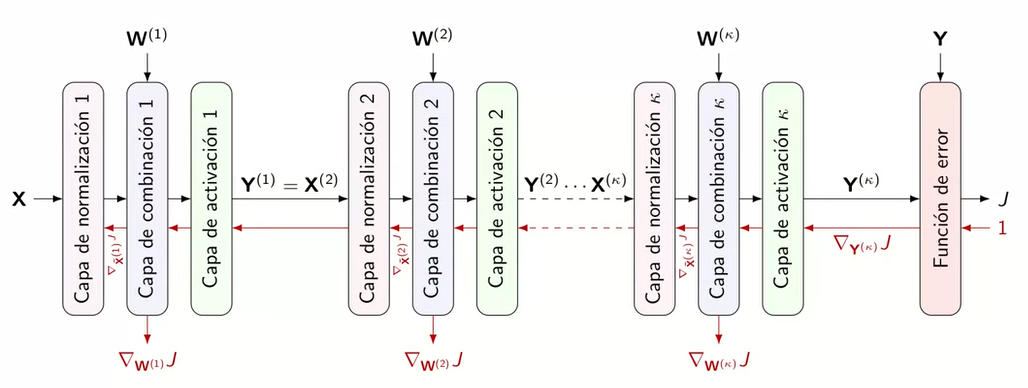
\includegraphics[width=\textwidth]{im1}
\end{frame}
%%%%%%%%%%%%%%%%%%%%%%%%%%%%%%%%%%%%%%%%%%%%%

\begin{frame}
  \frametitle{Contenido}

  \begin{itemize}
  \item Capas de combinación o transferencia
   \begin{itemize}
  \item Capas totalmente conectadas
  \item Capas convolucionales
  \end{itemize}
  \item Capas de activación
  \begin{itemize}
  \item Capas simples
 	\begin{itemize}
  \item Problemas: asimetría postiva, desvanecimiento del gradiente
  \end{itemize}
  \end{itemize}
  \item Normalización
  \item Funciones de pérdida
  \begin{itemize}
  \item MSE
  \item Entropía cruzada
  \end{itemize}
  \end{itemize}
\end{frame}
%%%%%%%%%%%%%%%%%%%%%%%%%%%%%%%%%%%%%%%%%%%%%
\section{Capas de combinación}
\subsection{Capa totalmente conectada}
\begin{frame}
  \frametitle{Capa totalemente conectada o densa}
  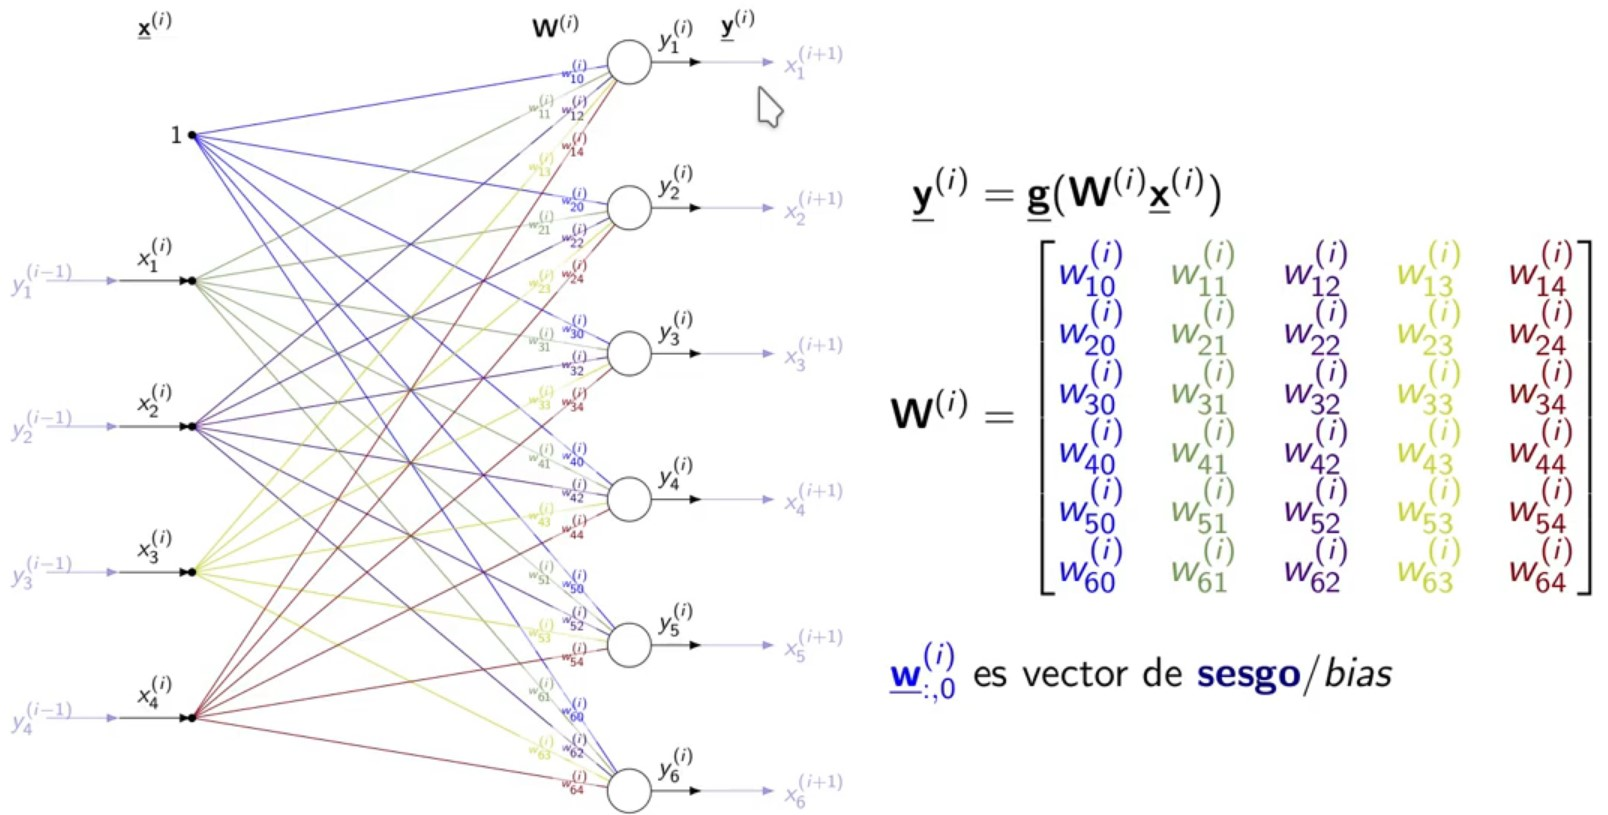
\includegraphics[width= \textwidth]{im2}
  
\end{frame}
%%%%%%%%%%%%%%%%%%%%%%%%%%%%%%%%%%%%%%%%%%%%%
\begin{frame}
  \frametitle{Capa totalemente conectada o densa}
\begin{itemize}
\item Estas capas producen $\boldsymbol{y}$ con una entrada $\boldsymbol{x}$ como combinación lineal:
\begin{equation*}
\boldsymbol{y}=\boldsymbol{W} \begin{bmatrix} 1 \\ \boldsymbol{x} \end{bmatrix}
\end{equation*}
\item Concepto se generaliza para procesar mini-lotes para matriz de diseño $\boldsymbol{X}$ con los datos en sus filas (y salidas en filas de $\boldsymbol{Y} $) 
\begin{equation*}
\boldsymbol{Y}= \begin{bmatrix} \textbf{1} & \boldsymbol{X} \end{bmatrix} \boldsymbol{W}^T
\end{equation*}
\item Generalmente utilizadas con datos de información distribuida en todas las componentes (salida múltiples de sensores) 
\end{itemize}
  
\end{frame}
%%%%%%%%%%%%%%%%%%%%%%%%%%%%%%%%%%%%%%%%%%%%%
\begin{frame}
  \frametitle{Inicialización de pesos}
\begin{itemize}
<<<<<<< HEAD
 \item ¿Cómo inicializamos las matrices $\boldsymbol{W}$?
 \begin{itemize}
 \item No es simple  de responder
 \end{itemize}
 \item Dependerá de los tipos de capas de activación que usamos
 \item Usualmente serán números aleatorios distribuidos de cierta forma 
 \item El rango de valores utilizables es limitado
 \item Si se eligen muy pequeños, el entrenamiento los aniquila ($\rightarrow 0$)
 \item Si se eligen muy grandes, explotan (NaN)
 \item Buena elección acelera convergencia 
 \item Marcos de trabajo ofrecen alternativas "estándar", pero cada método tiene un uso particular  
 \end{itemize}
=======
\item ¿Cómo inicializamos las matrices de pesos $\boldsymbol{W}$?

\item Dependerá de los tipos de capas de activación que usemos
\item Usualmente serán números aleatorios distribuidos de cierta forma.
\item El rango de valores utilizables es limitado
\item Si se eligen muy pequeños, entrenamiento los aniquila ($\rightarrow 0$)
\item Si se eligen muy grandes, explotan (NaN)
\item Buena elección acelera convergencia
\item Mala elección frena convergencia 
\item Marcos de trabajo ofrecen alternativas "estándar", pero cada método tiene un uso particular    
\end{itemize}
>>>>>>> 8d8dd1bffc7bc179ef89183b5d1e2e376e754ebe
  
\end{frame}
%%%%%%%%%%%%%%%%%%%%%%%%%%%%%%%%%%%%%%%%%%%%%
\begin{frame}
  \frametitle{Inicialización en capa totalmente conectada}
\begin{itemize}
<<<<<<< HEAD
 \item Asumamo que 
 \begin{itemize}
 \item entrada  $\boldsymbol{x}$ tiene componentes i.i.d.  $x_i~\mathcal{N}(0\sigma_x)$
 \item entrada  $\boldsymbol{W}$ tiene componentes i.i.d.  $w_{ij}~\mathcal{N}(0\sigma_w)$
 \end{itemize}
 \item Si $\boldsymbol{y}=\boldsymbol{W}\boldsymbol{x}$ ¿cómo se distribuyen los $y_i$?
 \item Para responder esto necesitamos dos propiedades: 
 \begin{equation*}
  E\left[   \sum_i a_i    \right] =\sum_i E \left[  a_i \right] 
 \end{equation*}
  \begin{equation*}
  E\left[   \prod a_i    \right] =\prod_i E \left[  a_i \right] 
 \end{equation*}
 siempre que $a_i$ sea independiente 
 \item Se cumple que $y_i=\boldsymbol{w}_{i,:}^T\boldsymbol{x}= \sum_{k=1}^{n}w_{ik}x_k$
 particular
 \end{itemize}
  
\end{frame}
=======
\item Asumamos que 
\begin{itemize}
\item entrada $\boldsymbol{x}$ tiene componentes i.i.d. $x_i \sim \mathbf{N}(0,\alpha_x)$
\item pesos $\boldsymbol{W}$ tiene componentes i.i.d. $w_ij \sim \mathbf{N}(0,\alpha_w)$
\end{itemize}
\item Si $\boldsymbol{y}=\boldsymbol{W}\boldsymbol{x} $ ¿cómo se distribuyen los $y_i$?
\item Para responder esto necesitamos dos propiedades: 
\begin{equation*}
E\left[ \sum_{i} a_{i}  \right] =\sum_i E \left[ a_{i}  \right]
\end{equation*}
\begin{equation*}
E\left[ \prod_{i} a_{i}  \right] =\prod_i E \left[ a_{i}  \right]
\end{equation*} siempre que $a_i$ sean independientes entre sí 
\item Se cumple que $y_i=\boldsymbol{w}_{i,:}^T\boldsymbol{x}=\sum_{k=1}^{n} w_{ik}x_k$
\end{itemize}
\end{frame}

>>>>>>> 8d8dd1bffc7bc179ef89183b5d1e2e376e754ebe
%%%%%%%%%%%%%%%%%%%%%%%%%%%%%%%%%%%%%%%%%%%%%
\begin{frame}
  \frametitle{Inicialización en capa totalmente conectada}
\begin{itemize}
<<<<<<< HEAD
 \item Valor esperado para $y_i$ es entonces
 \begin{equation*}
 E\left[   y_i  \right]= E\left[   \sum_{k=1}^n w_{ik}x_k    \right]=\sum_{k=1}^n E\left[ w_{ik} x_k  \right] =\sum_{k=1}^n E\left[ w_{ik}\right] E\left[ x_k  \right]=0
 \end{equation*}
 es decir, el valor medio sigue siendo cero
 \item la varianza de $y_i$ es (considerando que $E[y_i]=0$)
  \begin{equation*}
  \begin{split}
  Var[y_i]& = E\left[  (y_i-E[y_i])^2   \right] = E [y_i^2]= E\left[ \left(  \sum_{k=1}^n w_{ik} x_k \right)^2  \right]\\
  & = E\left[ \left(  \sum_{k=1}^n w_{ik} x_k \right) \left(  \sum_{k=1}^n w_{ik} x_k \right)  \right]=E\left[\sum_{k=1}^n \sum_{l=1}^n  w_{ik} x_k w_{il} x_l \right] 
  \end{split}
 \end{equation*}

 \end{itemize}
  
\end{frame}
%%%%%%%%%%%%%%%%%%%%%%%%%%%%%%%%%%%%%%%%%%%%%
\begin{frame}
  \frametitle{Inicialización en capa totalmente conectada}

  \begin{equation*}
  \begin{split}
  & = E\left[ \left(  \sum_{k=1}^n w_{ik} x_k \right) \left(  \sum_{k=1}^n w_{ik} x_k \right)  \right]=E\left[\sum_{k=1}^n \sum_{l=1}^n  w_{ik} x_k w_{il} x_l \right]\\
   &= \sum_{k=1}^n \sum_{l=1}^n E\left[w_{ik}  w_{il} x_k x_l \right] =\sum_{k=1}^n \sum_{l=1}^n E\left[w_{ik}w_{il} \right]E\left[  x_k x_l \right]
  \end{split}
 \end{equation*}
donde $x_k$ y $x_l$ son i.i.d solo si $k\neq l$, y lo mismo para $w_{ik}$ y $w_{il}$
\begin{itemize}
\item Esto quiere decir que si $k\neq l$ entonces $E[w_{ik}w_{il} ]=0$ y $E[x_k x_l ]=0$ 
\begin{equation*}
  \begin{split}
Var[y_i] & = \sum_{k=1}^n \sum_{l=1}^n E\left[w_{ik}w_{il} \right]E\left[  x_k x_l \right]=\sum_{k=1}^n E\left[w_{k}^2\right] E\left[  x_k^2\right]\\
& = \sum_{k=1}^n \alpha^2_w \alpha^2_x=n \alpha^2_w \alpha^2_x
\end{split}
\end{equation*}
=======
\item El valor esperado para $y_i$ es entonces 
\begin{equation*}
E\left[ y_{i}  \right] =E\left[ \sum_{k=1}^{n}{ w_{ik}x_{k} } \right]= \sum_{k=1}^{n}{ E\left[w_{ik}x_{k} \right]}=\sum_{k=1}^{n}{ E\left[w_{ik}\right]  E\left[x_{k} \right]}=0
\end{equation*}
es decir, el valor medio sigue siendo cero. 


\item La varianza de $y_i$ es (considerando que $E\left[ y_{i}  \right] =0$) 

\begin{equation*}
\begin{split}
Var\left[ y_{i} \right] & = E \left[ (y_{i}- E\left[ y_{i})^2 \right] )  \right]=E\left[ y_{i})^2\right]=E \left[ \left( \sum_{k=1}^{n}{ w_{ik}x_{k} }\right)^2   \right] \\
&=  E \left[ \left( \sum_{k=1}^{n}{ w_{ik}x_{k} }\right) \left( \sum_{l=1}^{n}{ w_{il}x_{l} }\right) \right]=   \sum_{k=1}^{n}\sum_{l=1}^{n} E \left[{ w_{ik}x_{k} } \right]  E \left[w_{il}x_{l}  \right]
\end{split}
\end{equation*}

>>>>>>> 8d8dd1bffc7bc179ef89183b5d1e2e376e754ebe
\end{itemize}
\end{frame}
%%%%%%%%%%%%%%%%%%%%%%%%%%%%%%%%%%%%%%%%%%%%%
\begin{frame}
  \frametitle{Inicialización en capa totalmente conectada}
<<<<<<< HEAD
\begin{itemize}
\item Si la entrada tiene $\alpha_x=1$, entonces $Var[y_i]=n\sigma^2_w$
\item Si pegáramos varias capas, la varianza ¡crece con n!
\item luego de varias capas, esos números alcanzarían NaN
\item Si queremos que $Var[y_i]=1$ entonces tenemos que elegir $\sigma_w=1/\sqrt{n}$
\item El análisis anterior solo considera la capa conectada  aislada
\item Falta considerar la capa de activación 
\item Salida de esa capa debería tener varianza unitaria (entrada a siguiente capa)
\end{itemize}

\end{frame}
%%%%%%%%%%%%%%%%%%%%%%%%%%%%%%%%%%%%%%%%%%%%%


=======


\begin{equation*}
\begin{split}
&=  E \left[ \left( \sum_{k=1}^{n}{ w_{ik}x_{k} }\right) \left( \sum_{l=1}^{n}{ w_{il}x_{l} }\right) \right]=   \sum_{k=1}^{n}\sum_{l=1}^{n} E \left[{ w_{ik}x_{k} } \right]  E \left[w_{il}x_{l}  \right]\\
&=  \sum_{k=1}^{n}\sum_{l=1}^{n}E \left[w_{ik}w_{il}x_{k}x_{l}\right]=\sum_{k=1}^{n}\sum_{l=1}^{n} E \left[w_{ik}w_{il}\right]E \left[x_{k}x_{l}\right]
\end{split}
\end{equation*}
donde $x_k$ y $x_l$ son i.i.d. solo si $k\neq l$, y lo mismo para $w_{ik}$ y $w_{il}$ 

\end{frame}
%%%%%%%%%%%%%%%%%%%%%%%%%%%%%%%%%%%%%%%%%%%%%
>>>>>>> 8d8dd1bffc7bc179ef89183b5d1e2e376e754ebe

\begin{frame}
  \frametitle{Inicialización en capa totalmente conectada}

\begin{itemize}
\item Esto quiere decir que si $k\neq l$ entonces $E \left[w_{ik}w_{il}\right]=0 $ y $E \left[x_{k}x_{l}\right]=0$
\begin{equation*}
Var\left[ y_{i} \right] = \sum_{k=1}^{n}\sum_{l=1}^{n} E \left[w_{ik}w_{il}\right]E \left[x_{k}x_{l}\right]= \sum_{k=1}^{n}E \left[w_{ik}^2\right]E \left[x_{ik}^2\right]= \sum_{k=1}^{n}\sigma_{w}^2 \sigma_{x}^2
\end{equation*}¨
\begin{equation*}
 \sum_{k=1}^{n}\sigma_{w}^2 \sigma_{x}^2= n\sigma_{w}^2 \sigma_{x}^2
\end{equation*}
\item si la entrada tiene $\sigma_x=1$, entonces $Var[y_i]=n\sigma_{w}^2$
\item Si pegáramos varias capas, la varianza !crece con! (números posibles van a crecer)
\item Luego de varias capas, esos números alcanzarían NaN
\item Si queremos que $Var[y_i]=1$ entonces tenemos que elegir $\sigma_w=1/\sqrt{n}$ 
\end{itemize}
\end{frame}
%%%%%%%%%%%%%%%%%%%%%%%%%%%%%%%%%%%%%%%%%%%%%

\begin{frame}
  \frametitle{Inicialización en capa totalmente conectada}

\begin{itemize}

\item El análisis anterior solo considera la capa conectada aislada 
\item Falta considerar la capa de activación
\item Salida de esa capa debería tener varianza unitaria (entrada a siguiente capa)
\end{itemize}
\end{frame}
%%%%%%%%%%%%%%%%%%%%%%%%%%%%%%%%%%%%%%%%%%%%%

\begin{frame}
  \centering \LARGE
  \emph{Capas convolucionales}
\end{frame}
%%%%%%%%%%%%%%%%%%%%%%%%%%%%%%%%%%%%%%%%%%%%%

%%%%%%%%%%%%%%%%%%%%%%%%%%%%%%%%%%%%%%%%%%%%%
\end{document}


%\end{document}

%%% Local Variables:
%%% mode: latex
%%% TeX-master: t
%%% End:
